\chapter{Experiencias y mediciones realizadas}
\label{simulations}
En este capítulo se presentan las mediciones del sistema completo así como de módulos aislados. 
En la primera parte se muestran los resultados del simulador numérico, para después detallar mediciones en las implementaciones completas realizadas, utilizando un medio óptico y luego un medio acústico.
\section{Implementación en software}
Como paso previo a realizar las implementaciones sobre FPGA en el caso óptico, y sobre software en el caso acústico, simuladores numéricos de todas las etapas fueron implementados y combinados para corroborar los resultados teóricos. Esta implementación fue realizada utilizando el lenguaje de C/C++. Es necesario utilizar este tipo de lenguaje de alto rendimiento debido a que se necesitan simular grandes cantidades de datos para realizar mediciones de tasas de error del orden de 10e-8. Específicamente, en cada corrida se simula la transmisión de > 1 Gb de datos por cliente, con hasta 128 clientes, por lo que se requiere de la mayor rendimiento posible para obtener tiempos aceptables.

\subsection{Estructura general}

La estructura general del simulador es modular, con una separación de alto nivel que obedece al diagrama lógico que puede verse en la figura \ref{fig_comstack}.
Cada módulo representa una etapa en el sistema de comunicaciones que realiza una transformación específica sobre los datos, que puede ser modulación, demodulación, corrección de errores, etc. Los diferentes módulos actúan como filtros, recibiendo y enviando los datos transformados utilizando la entrada y salida estándar del sistema operativo (STDIN/STDOUT). La simulación comienza con un bloque generador de datos binarios aleatorios. Estos datos son alimentados a la primer etapa, que es el módulo de corrección de errores. La salida codificada es entonces alimentada a la siguiente etapa, y de esta manera, los datos originales son sucesivamente transformados en cada módulo.

El medio de transmisión físico es también simulado mediante un módulo de que agrega ruido de acuerdo a las características del canal seleccionado. Por ejemplo, en el módulo de simulación óptica se tiene en cuenta la dispersión y atenuación de la señal sobre una fibra óptica.

Al llegar a la última etapa de la recepción, donde deberían obtenerse los datos originales, el resultado es comparado bit a bit con los datos introducidos originalmente, y en base a las diferencias detectadas se calcula y reporta el BER.

Esta estructura modular brinda flexibilidad al simulador, permitiendo introducir y remover etapas fácilmente.

Citaremos rápidamente cada módulo y sus parámetros:
\begin{description}
 \item[rsenc/rsdec] Codificador/Decodificador de la etapa de corrección de errores. Específicamente se implementa el algoritmo Reed-Solomon 223/255. Se puede generar un código ``recortado'' especificando la cantidad de bytes por bloque en el primer argumento.
 \item[scrambler/descrambler] Implementación del scrambler de datos. El tamaño de bloque puede ser especificado en el primer argumento. Es recomendable que el tamaño de bloque sea un múltiplo del tamaño de bloque del corrector de errores (en nuestro caso, 255 bytes).
 \item[bfenc/bfdec] Etapa codificadora/decodificadora que utiliza el filtro de Bloom. En esta etapa se agregan los demás clientes a simular, cuyos datos son generados aleatoriamente. El único argumento es la cantidad de clientes presentes en el canal.
 \item[noisesim] Simulador de ruido óptico, donde se distorsiona el bit transmitido de acuerdo con la velocidad y parámetros de la fibra óptica simulada. La velocidad esta fija a 10 GB/S. El único parámetro especifica la cantidad de clientes interfiriendo la señal.
\end{description}

En general, el simulador puede correr cada etapa consecutivamente, donde cada módulo completara el procesamiento de datos antes de comenzar con la próxima etapa:

\small
\begin{verbatim}
 ./rsenc <${FILE} | ./scrambler ${SCRAMBLEBLOCK} >rs.out
 ./bfenc ${CLIENTES} < rs.out | ./noisesim -c ${CLIENTES} -r 16.6 >bfenc.out
 ./bfdec ${CLIENTES} <bfenc.out >bf.out
 ./descramble ${SCRAMBLEBLOCK} <bf.out | ./rsdec >rsdec.out
\end{verbatim}
\normalsize
Notar en el ejemplo anterior que los módulos utilizan archivos temporales como forma de comunicación.

Una simple modificación en la manera de ejecutar los módulos alimenta la salida de un módulo directamente a la entrada del módulo siguiente, sin necesitar archivos temporales y ejecutándose en forma paralela:
\small
\begin{verbatim}
./rsenc <${FILE} | ./scrambler ${SCRAMBLEBLOCK} | ./bfenc ${CLIENTES} | \
                 ./noisesim -c ${CLIENTES} -r 16.6 | ./bfdec ${CLIENTES} | \ 
                 ./descramble ${SCRAMBLEBLOCK} | ./rsdec > file.out
\end{verbatim}
\normalsize

En la primera configuración del simulador, se puede acceder a los archivos temporales intermedios, útiles para depuración y mediciones por etapa, mientras que la segunda configuración tiene la ventaja de aprovechar la totalidad de los procesadores disponibles en el sistema, ya que en un sistema multi-procesador, el sistema operativo usualmente asigna un CPU a cada etapa y estas se ejecutan en paralelo.

La implementación sobre medio acústico no presenta mayor inconveniente ya que las tasas de transmisión son bajas, acotadas naturalmente por el medio de transmisión y ancho de banda disponible, por lo que los recursos computacionales necesarios para la simulación son limitados. Otro caso es la simulación del medio óptico, donde normalmente se necesita simular una transmisión de 10e9 bits o más para obtener una medición confiable del BER del sistema, ya que este medio tiene naturalmente una tasa elevada y un BER muy reducido. Adicionalmente, sobre este medio el sistema soporta un máximo de 128 clientes que son simulados simultáneamente, por lo que los recursos computacionales requeridos son considerables. A raíz de este problema, y aprovechando que la simulación es altamente paralelizable, se implementó un sistema de estilo cliente-servidor donde los cálculos son distribuidos en un grupo de múltiples nodos.

\subsection{Etapa de corrección de errores/Scrambler}

Los módulos de corrección de errores (rsdec/rsenc) y scrambler (scrambler/descrambler) fueron implementadas utilizando bibliotecas de código abierto, mientras que el scrambler/descrambler es un algoritmo trivial y de rápida codificación. Se utilizó la popular biblioteca libFEC del autor Phil Karn \cite{libfec}. El algoritmo de scrambling utiliza una matriz de permutación aleatoria que es generada mediante una semilla en cada ejecución, garantizando que las permutaciones sean reversibles.

\subsection{Implementación de filtro de Bloom}
El módulo bfenc/bfdec realiza la codificación/decodificación por software del algoritmo de filtro de Bloom. Los parámetros del algoritmo tales como el tamaño del filtro $M$ y la cantidad de clientes a simular son configurables. Una característica que merece mencionarse es el sistema de minimización de peso de Hamming que es realizada en esta etapa. Tal como se explica en \ref{miniham}, la  implementación se realiza mediante una tabla de lookup (ver tabla \ref{hwtable}), lo que permite consultas muy eficientes con una complejidad temporal de $O(1)$, aunque el tamaño de la tabla (también llamado complejidad espacial del algoritmo) se aproxima a $O(2^{N})$ con $N$ siendo la cantidad de bits por símbolo, por lo que para tamaños razonables de $N<24$ es autogenerada en cada ejecución en función de los parámetros necesarios.

\subsection{Simulador de medio acústico}

El medio de transmisión acústico fue simulado adoptando un modelo físico relativamente sencillo, que solo toma en cuenta ciertas limitaciones en la respuesta en frecuencia. Para esto se crearon módulos independientes que realizan la modulación, sincronización, demodulación y filtrado de la señal resultante.
Los módulos transforman los bits de entrada en una señal de audio digital con codificación PCM (\textit{Pulse Coded Modulation}), a las cual se aplica un filtro pasa banda para simular las limitaciones en frecuencia de los transductores, como pueden ser los parlantes y micrófonos de un dispositivo móvil. Este módulo respeta el diseño de los anteriores, emitiendo la señal analógica como un flujo de bytes con codificación PCM vía la salida estándar del sistema. El filtro pasa banda fue implementado como un filtro digital de respuesta finita o FIR.
Este simulador utiliza algoritmos de modulación, filtros y sincronizacíon reales, por lo que muchos módulos pudieron ser utilizados sin modificaciones en un medio real. Para mas detalles de estos módulos, ver sección \ref{redacus}.

\subsection{Simulador de ruido óptico}
%% de orte.text

El modelo de simulación del canal óptico toma en cuenta tanto efectos lineales como no-lineales en la fibra óptica. Los pasos de la simulación son los siguientes:

Se asume que el tráfico proveniente de todas las ONUs alcanza al divisor de $128\times1$ con perfecta sincronización de bit, o sea, sin fluctuaciones o \textit{jitter}.
Los slots correspondientes al bit `0' contienen una pequeña intensidad óptica de CW (\textit{Continous Wave, potencia siempre presente en el Laser}) dada por el razón de extinción de Tx.
Debido a esta potencia óptica siempre presente, cada ONU agregado al sistema agrega una pequeña intensidad de bit `0', incrementando la potencia base total (ver figura \ref{sim:extinction}).
Para la simulación se asume que cada bit `1' agrega un pulso super-Gaussiano ($m=4$) al nivel de potencia base, con un ciclo de trabajo (duty cycle) de $1/3$, una aproximación razonable a los parámetros utilizados por el transceptor de gigabit utilizado.

\begin{figure}[!t]
    \centering
      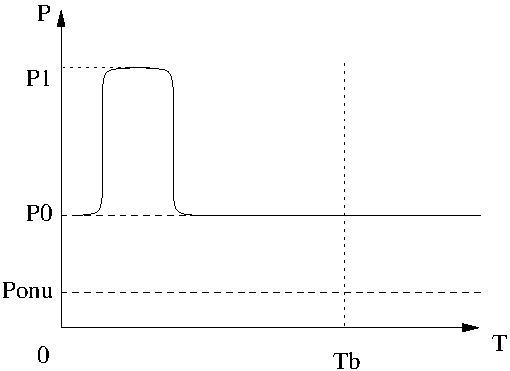
\includegraphics[width=3.5 in]{graphs/extinction.pdf}
      \caption{Diagrama de un bit ideal. Observar que la potencia del nivel del cero no equivale a potencia cero, sino a $P_0$, que se define como $P_0=Ponu*N$ donde N es la cantidad ONUs activas.}
      \label{sim:extinction}
\end{figure}

%The physical optical channel simulation block provides an estimate of
%the BER performance of the optical channel. Simulation steps are as
%follows: RZ upstream traffic coming from all ONUs is assumed to arrive
%at the $128\times1$ splitter with perfect time synchronization, i.e., there is no timing jitter. 
%This allows to simulate merged traffic as a simple addition of optical intensities at bit slots for either `0' or `1' bits. % borrar!
%The `0'-bit slots contain a small CW optical intensity given by the Tx extinction ratio. 
%Each on-line ONU adds its `0'-bit optical intensity yielding a base power level.
% As many bit `0' optical intensities are added as on-line ONUs to produce a base power level.  
%Each `1'-bit adds a super-Gaussian ($m=4$) pulse, duty cycle $1/3$, to the base power level. %, with rising edge at slot start and peak amplitude accordingly to Tx optical mean output power.
% As many bit `1' intensities are added to base level as active Tx there are at each simulation bit slot.

Tanto el tráfico saliente como el entrante sufren atenuaciones debido a múltiples factores que incluyen pérdidas en el divisor, fibra y empalme (\textit{splice}). El presupuesto de potencia (\textit{power budget}) se balancea mediante un EDFA (\textit{erbium-dopped fibre amplifier}) con una ganancia constante de $27$~dB, valór calculado como el necesario para contrarrestar las pérdidas totales sobre un enlace de 10Km. Un factor en el incremento del BER sobre enlaces ópticos es  la emisión espontánea amplificada del amplificador EDFA. Este parámetro es modelado como ruido blanco gaussiano, con una intensidad proporcional a la figura de ruido del amplificador ($7$~dB), y es agregada luego del modelado del EDFA.

%Upstream and downstream merged traffic suffers from attenuation due to
%splitter, fiber, and
%splice losses. The power budget is balanced by an EDFA with $27$~dB constant gain.
%Amplified spontaneous emission from the EDFA is modeled by white Gaussian
%noise, with intensity proportional to the amplifier noise figure ($7$~dB), and is added
%after the EDFA. 

%Real EDFAs gain increases with higher input power, i.e. amplification is not
%linear with number of active Txs. Settling for worst case scenario simulation
%we assume same $27\,dB$ gain for any number of active Txs. ASE noise produced
%at EDFA is modelled as a white Gaussian noise added to the optical signal. An
%EDFA accomplishing the amplification previously discussed ($-25.5\,dBm$ to
%$1.5\,dBm$) would have an output SNR $\geq 60\,dB$ accordingly to a estimation
%based on the bandwidth of forthcoming optical filtering at APD detector (see
%section 6.5.1 at~\cite{Agrawal:xx}). Dispersion compensation regeneration stage
%operation is accounted for by simulating no dispersion effects. Traffic is
%routed back to all ONUs by a 1x128 splitter through another $10\,km$
%fiber,
%amounting to a $27.5\,dB$ attenuation; so for one active Tx input power at each
%Rx would be $-27\,dBm$.

La señal de entrada óptica al receptor es filtrada con un filtro Butterworth de segundo orden y $25$~GHz de ancho de banda, para luego simular su deteccion asumiendo la respuesta de un dispositivo PD (\textit{photodiode}) estándar (ver sección 4.4.3 de ~\cite{Agrawal:xx}).
Finalmente, para simular el ruido térmico y ruido de disparo o \textit{shot}, se agrega un componente de ruido blanco gaussiano.

%The input optical signal at the receiver is filtered (2nd order low-pass Butterworth filter, $25$~GHz bandwidth) and photodetected assuming a standard PD responsivity (see section 4.4.3 of~\cite{Agrawal:xx}).
%White Gaussian noise accounting for thermal and shot noise is then added
%to the photocurrent, and 
%electrical filtering is applied (2nd order low-pass Butterworth filter, $14$~GHz bandwidth).
%Simulating the decision process a mean of samples around maximum eye opening is compared to a threshold current. 
%Current in case of `1' bits collision is higher than that of a single active Tx, so threshold is established assuming that later case.

%Real EDFAs gain increases with higher input power, i.e., amplification would not be linear with number of active Txs. 
%Settling for worst case scenario simulation we assume same $27\,dB$ gain for any number of active Txs. 
%ASE noise produced at EDFA is modeled as a white Gaussian noise that's added to the electric field. 
%An EDFA accomplishing the amplification previously discussed ($-25.5\,dBm$ to  $1.5\,dBm$) would have an output SNR $\geq 100\,dB$ accordingly to a estimation based on the bandwidth of forthcoming optical filtering at detector (see section 6.5.1 at~\cite{Agrawal:xx}). 
%Effect on traffic of dispersion compensation regeneration stage is accounted by not including in the simulation pulses deformation due to dispersion. 
%Afterwards traffic is routed back to all ONUs by a $1\times128$
%splitter through another $10\,km$ fiber, amounting to a $27.5\,dB$ attenuation arriving to each Rx with $-27\,dB$ for one active Tx.
%
%A concern was if maximum mean total input power allowed at Rx would be surpassed when multiple Tx were simultaneously active. 
%Simulation shown that the occurrence of 15 simultaneously active Tx was a very rare event {\bf <CUANTO??>}. 
%That would amount to $\sim-15\,dBm$ reaching each ONU Rx, well bellow standard commercial Rx overload of $\sim+0.5\,dBm$, that's maximum acceptable mean input power for a BER$<1\,10^{-12}$. 
%
%Rx optical bandwidth is simulated as a low pass filter (2nd order Butterworth as a digital IIR filter~\cite{IIR}, cutoff frequency $25\,GHz$). Afterwards optical traffic is converted into an electrical current. Then to account for thermal and shot noise at a typical APD white Gaussian noise current is added, with an estimated SNR $\simeq 42\,dB$ (see section 4.4.3 at~\cite{Agrawal:xx}). Then electrical filtering is applied (2nd order Butterworth IIR filter, cutoff frequency $6\,GHz$). Detection procedure is performed by comparison to a fixed current threshold. A previous simulation run with the same number of ONUs but with a single active Tx allows to determine the decision threshold at the time of maximum eye diagram opening. Addition of bit `1' amplitudes (collision) produce a current even higher than for a single active Tx, thus this bit slot will be classified as `1' at optical channel simulation output. 
%Media block account for fiber, EDFA and splitters. It attenuates optical trains (splitters and fiber attenuation minus EDFA gain) and also adds white Gaussian noise to the electric field accounting for ASE noise at EDFA. 
% MUCHO, MUY IMPORTANTE: REVISAR CALCULO OSNR (Fn) y verificar que se determina en detector %[VAB]
% ITU recommendation G. 959.1 states that certain interfaces' should operate normally up to $12\,dBm$ mean total input power. In any case if such power is surpassed it would only cause a very short time blinding of Rx affecting a so small amount of bits that wouldn't affect the logical layer ability to correct them.
% receiver overload: max input power for BER<1E-12
%Receiver block simulates Rx behavior. It's optical bandwidth is taken into account by simulating a low pass filtering of incoming traffic (2nd order Butterworth as a digital IIR filter~\cite{IIR}, cutoff frequency $25\,GHz$). Then optical traffic is converted into an electrical current. White Gaussian noise current is added to account for thermal noise at Rx, being it's SNR $\simeq 42\,dB$ accounting for thermal and shot noise at a typical APD detector (see section 4.4.3 at~\cite{Agrawal:xx}). Afterwards another filter simulates detector's linear channel (2nd order Butterworth IIR filter, cutoff frequency $6\,GHz$). Detection procedure is performed by comparison to a fixed current threshold. A previous simulation run with same number of ONUs but with a single active Tx allows to determine the decision threshold at the time of maximum eye diagram opening. Addition of bit `1' amplitudes (collision) produce a current even higher than for a single active Tx, thus this bit slot will be classified as `1' at 
optical channel simulation output. 


\section{Redes ópticas}
La implementación del sistema sobre redes ópticas fue el objetivo principal de la investigación.
La simulación tuvo un papel muy importante en el desarrollo y pruebas del algoritmo en este medio debido a las elevadas tasas de transmisión involucradas (el transceptor utilizado puede utilizarse a un mínimo de 1 Gbps y máximo de 9.33 Gbps), valores que prohiben las mediciones directas por medio de un osciloscopio u herramientas similares. Sin embargo ciertos valores tales como el ancho de bit y radio de extinción pueden obtenerse mediante observación directa del diagrama de ojo de la señal.

\subsection{Simulaciones numéricas}

Podemos citar dos resultados importantes obtenidos mediante las simulaciones numéricas. 
En el primero, detallado en la Fig.~\ref{sim:optical}, se muestra que nivel de razón de extinción mínimo requerido para lograr un BER arbitrario es directamente proporcional al número de ONUs presentes on-line.
Podemos deducir de este gráfico que mientras mas ONUs utilizen el sistema, se necesitaran Lasers con un radio de extinción mas elevado. Además, con una mayor cantidad de ONUs, se incrementa el BER por problemas físicos: Las fluctuaciones a niveles de potencia cercanos al límite de sensibilidad del dispositivo PD tienen un importante efecto en la detección de la señal.
El ruido de shot es particularmente preocupante ya que es proporcional al la fotocorriente media. En nuestra propuesta, este ruido es mas alto que en PONs comunes ya que la intensidad del bit `0' de todas las ONUs presentes contribuyen al mismo.
%Noise fluctuations at power levels near the PD sensitivity limit have an important effect on signal detection. 
%Detection being made at power levels near PD sensitivity is highly sensitive to changes in noise.
%Shot noise is of particular concern as it is proportional to the mean photocurrent.
%In our network proposal the later is higher than in PONs as bit
%`0' optical intensities from all ONUs are added.
%The resulting base-level optical intensity is then heavily dependent on the Tx extinction ratio.
%Fig.~\ref{sim:optical} shows minimal extinction ratios required to
%achieve an arbitrary BER in the physical layer as a function of the
%number of on-line ONUs.
\begin{figure}[!t]
    \centering
      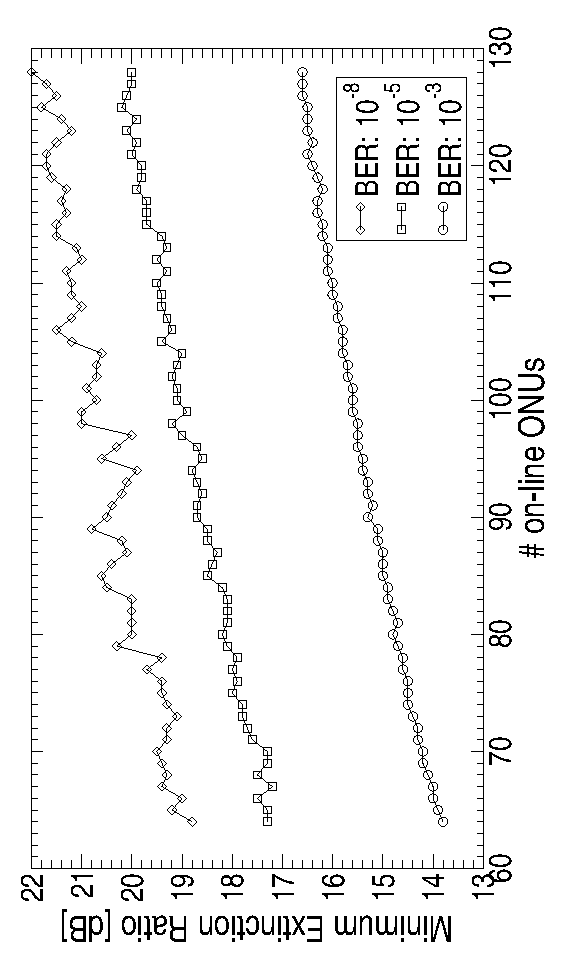
\includegraphics[angle= 270, width=3.5 in]{graphs/orte03.pdf}
%      \caption{Physical layer simulation result: Minimal extinction ratio required to assure a given BER}
      \caption{Resultado de simulaciones de la capa física: razón de extinción mínimo requerido para asegurar un cierto BER.}
      \label{sim:optical}
\end{figure}
En el escenario de $128$ ONUs presentes, un BER menor a 10e-3 puede ser logrado utilizando transmisores del tipo comercial con un razón de extinción de $\simeq16.6$~dB.
Este BER es lo suficientemente bajo para permitir rutinas de corrección de errores al nivel del canal lógico, que garanticen la transmisión libre de errores realizando una utilización acotada de la capacidad total del canal.
%In the $128$ ONUs scenario a  BER$<10^{-3}$ can be achieved using
%commercially available transmitters with an extinction ratio $\simeq16.6$~dB.
%This BER is low enough to allow for logical-channel error-correction routines that guarantee error-free transmission, while still making use of a fair fraction of channel capacity.
% perform correctly and still use a fair fraction of channel capacity.
% Fig.~\ref{sim:optical} shows simulation results for the BER vs OSNR
% for different numbers of ONUs with fixed electrical SNR $\simeq 42$~dB.
% Higher BERs as ONUs number increases due to the higher probability of
% simultaneous bit `1' transmissions (collisions) yielding pulses of
% optical power higher than that of a logical
% `1', generating intersymbol interference. Higher powers generate higher
% currents at Rxs that demand longer times to settle to logical `0' levels after
% filtering. Nevertheless, as
% can be seen in fig.~\ref{sim:optical}, in the worst case scenario (128
% ONUs) the expected OSNR at the EDFA output is enough ($\geq 40$~dB) to
% ensure a BER$<10^{-7}$. In this case simulation shown that the occurrence of
% 15 simultaneously active Tx was a very rare event, so optical power at Rx
% would be $\simeq -15$~dBm, well bellow standard commercial Rx overload
% of $\sim0.5$~dBm (maximum acceptable mean input power for a
% BER$<10^{-12}$).

\begin{figure}[t]
  \centering
  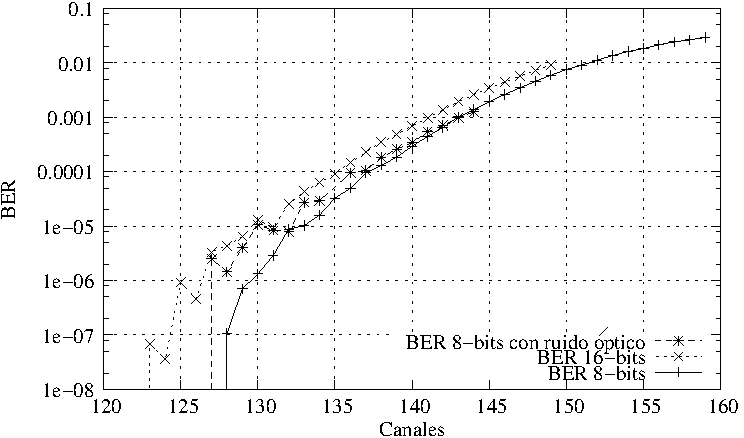
\includegraphics[width=4in]{graphs/BER-tesis.pdf} 
  \caption{BER del canal de un ONU a 10 Gbps Vs. la cantidad de ONUs activos.}
  \label{sim:access}
\end{figure}
aaaa

La Fig.~\ref{sim:access} muestra los resultados de la simulación del canal, comparando el BER de un ONU con respecto la número total de ONUs activos. Las dos primeras mediciones muestran la diferencia en rendimiento al utilizar símbolos de 8 bits contra símbolos de 16 bits, y la tercera para apreciar la diferencia en el resultado al agregar el ruido óptico dentro de la simulación.
Los resultados fueron obtenidos enviando un gigabit de datos por cada ONU simultáneamente. El mismo método se utilizó para realizar las simulaciones cuyo resultados se presentan en la Fig.~\ref{BERvsExpansion}, donde se aprecia una mejora de rendimiento importante al utilizar el algoritmo de reducción de peso de Hamming.
Volviendo a la Fig.~\ref{sim:access}, puede verse que cuando la cantidad de ONUs supera los 128, el BER se eleva marcadamente.
De la misma figura podemos observar una disminución de la capacidad en aproximadamente $8$ ONUs cuando el ruido de la capa óptica es agregado a la simulación, debido a la razón de extinción y el ruido producido por el EDFA y los PDs.
Finalmente, la carga máxima que soporta el sistema con un BER máximo de 10e-8 es del $90\%$, lo que significa que en una red de 128 clientes, es posible que 119 ONUs esten transmitiendo al mismo tiempo.


%Fig.~\ref{sim:access} shows simulation results for the fraction of the total
%capacity and the BER of one channel at the coding level (circles) and 
%including physical layer impairments (squares). 

%These results were obtained by
%sending one Gigabit of data for each ONU simultaneously.
%This figure shows a channel utilization of $15.7\%$ when all of $128$ ONUs
%are transmitting simultaneously, with a BER$<10^{-8}$. 
%From Fig. \ref{arch:fig1} we observe a penalty of $8$ ONUs when
%impairments from the optical layer (mainly extinction ratio and noise from EDFA and PDs) are taken into account.
%Considering that the system was designed to support asynchronous communications (e.g., Ethernet), it is not likely that all the ONUs will transmit simultaneously (e.g., Internet links often operate at most at $90\%$ load); and therefore our system has a BER $<10^{-8}$ for each channel when 119 ONUs are transmitting at a same time ($119/128>0.9$).
%, removing only one ONU re-establish the desired BER. 
%
%It is worth to remark that, even if the optical channel can induce a
%significant number of errors, the access layer has shown to be able to correct a
%very large number of errors (it is based on
%LDPC+Reed-Solomon+Bloom-Filters), as can be seen on the curve with squares
%at fig.~\ref{sim:access}.
%Observe that the high error rates correspond to a
%worst-case scenario when all ONUs are transmitting simultaneously at
%full capacity, and also 
%there is a low penalty due to physical layer impairments.
%Figure~\ref{sim:optical} presents the simulation's BER vs optical OSNR
%for different numbers of ONUs. %[VAB]
%As the number of ONUs increases higher BERs are obtained at the same optical SNR (electrical SNR is fixed at $\simeq 42\,dB$). In particular there is a penalty of about $30\;dB$ for 128 ONUs in comparison to 1 ONU. This is expected as a consequence of the higher probability of simultaneous bit `1' transmissions (collisions) yielding pulses (logical `1's) of different powers (sum of the power of each transmitter). Higher powers demand more time to settle post filtering current to logical `0' levels. If the following bit slot is indeed a logical `0' an erroneous determination is more possible with a higher collision probability. Nevertheless it can be inferred from simulation results that optical channel should not add significantly to the BER for the whole link as the estimated optical SNR of $\geq 100\,dB$ even for the worst case scenario with 128 ONUs present.
% \begin{figure}[!t]
%     \center
% %     \subfigure[Optical channel]{
% %      \label{sim:optical}
%       \includegraphics[scale=0.4]{BERvsSNR_6GHz.pdf}
% %    }
% %    \subfigure[Logical channel]{
% %      \label{sim:access}
%       \includegraphics[scale=0.4]{BERvsONUs.pdf}
% %    }
%     \caption{Simulation results}
%       \label{archfig}
% \end{figure}

\section{Implementación en FPGA}
El estudio de PONs plantea el desafío de generar, transmitir y recibir
señales de 10 Gbps en el laboratorio. El costo de estos sistemas
suele ser muy elevado. En este trabajo proponemos una alternativa de muy
bajo costo basada en la generación y trasmisión de señales utilizando dispositivos del tipo FPGA.

\subsection{Arquitectura alto nivel de la FPGA Xilinx ML507}
El equipamiento se compone de un kit de desarrollo ML-507 de Xilinx \cite{virtex5fpga} y un
transceptor SFP+ con varios emisores Láser XFP de 1330 nm y 1550 nm, con capacidad de hasta 10 Gbps
en modulación NRZ y alcance de 10km en fibra monomodo \cite{virtex5fpgaRIO}. Para realizar
las mediciones presentadas en este trabajo se utilizaron dos herramientas de medición:
\begin{itemize}
 \item Osciloscopio Óptico Agilent 86100A con módulo óptico 86105A: Para
realizar las mediciones físicas contamos con este equipo que posee un
ancho de banda óptico 20 Ghz, suficiente para capturar en
tiempo real los bits individuales o realizar un diagrama de ojo.
\item {\em Integrated Bit Error Rate Tester} (iBERT) \cite{4gtxs}: Este dispositivo es un medidor de tasa de error con interfaz para la herramienta de
verificación y depuración ChipScope \cite{arshak2006testing}. Esta herramienta puede denominarse ``virtual'' ya que consiste íntegramente en nucleos IP (\textit{intellectual preperty}) púramente lógicos, que deben ser sintetizados y embebidos junto con el diseño dentro de la FPGA.
Con iBERT es posible medir en tiempo real varios parámetros del transceptor asi como realizar estadísticas y mediciones de error, variando tasas y características de la transmisión en tiempo real.
 
\end{itemize}
\subsection{Transmisión a multi gigabit}
La plataforma de FPGA de Xilinx no fue seleccionada solamente porque la lógica programable es necesaria para la transmisión a altas velocidades, sino por la versatilidad y velocidad de los transceptores de multi gigabit incluidos en las mismas, esto es, la ``maquinaria'' necesaria para serializar/des-serializar y codificar bits de datos, asi como las interfaces para conectar las salidas directamente a las entradas de transceptores ópticos, como uno o más XFPs \cite{ug198}.

Los transceptores de multi gigabit estan preparados para operar sobre diversos medios físicos, como por ejemplo sobre cables trenzados de cobre o líneas de transmisión de alta velocidad sobre PCBs (\textit{printed circuit boards}). Serial-ATA y PCI-Express son protocolos de transmisión de datos que suelen ser implementados utilizando los transceptores de la FPGA. Sin embargo, en redes de comunicaciones PON se requieren alcances del orden de Kms, que solo pueden ser alcanzado mediante fibras ópticas.

\subsection{Diseño del sistema propuesto}
En la Fig.~\ref{fig:fpgadesign} puede observarse el diseño propuesto en el cual se implementó y probó exitosamente el algoritmo transmitiendo a tasas de 5 Gigabits mediante una fibra óptica.
Estas velocidades fueron logradas gracias a ciertas características del diseño que serán descritas a continuación.

A nivel de diseño digital, el sistema puede separarse en 4 módulos:

\begin{description}
 \item[Transceptor de gigabit:] este componente de hardware es provisto por la FPGA. Puede verse como un serializador/deserializador pero contiene mas de 15 subsistemas incluyendo buffers, PLLs (\textit{phase-locked loop}), codificadores y decodificadores. Adicionalmente, el transceptor posee herramientas para sincronización y depuración, permitiendo realizar mediciones y crear lazos de realimentación o \textit{loopbacks} en 3 puntos diferentes del flujo de datos para detectar anomalías. Se conecta a la lógica programable de la FPGA por medio de más de 200 señales de control y transferencia de datos, cuyas funciones son encapsuladas por un módulo especial de lógica que simplifica la interfaz con el resto del sistema. Esta lógica de interfaz se implementó como un módulo de Verilog, llamado ``v5\_gtxwizard\_v1\_7\_tile.v'' en el árbol de código fuente.

 \item[Generador de frame:] este módulo se encarga de codificar los datos a transmitir y enviarlos por el transceptor de gigabit. Contiene implementaciones de las etapas necesarias, tales como el codificador de RC4, Bloomfilter encriptado y expansión de peso de Hamming, así también como del sistema de sincronización de frame. La estructura interna es la de una máquina de estados finita, estando implementada íntegramente en lógica digital (sin utilizar ningún componente de software). Se implementó en un solo módulo de Verilog llamado ``frame\_gen.v''.
 
 \item[Decodificador de frame:] La contrapartida del generador del frame es el decodificador, que posee los decodificadores correspondientes tales como Reed-Solomon, RC4, Bloomfilter y expansión de peso de Hamming, así también como el sincronizador de frame y word, que utiliza parcialmente el hardware de sincronización del transceptor de gigabit para sincronizar a nivel de byte, sumado a una sincronización propia para lograr la sincronización a nivel de double-word y finalmente, sincronización de frame (ver sección \ref{fpga:sync}). La implementación también consiste de una sola maquina de estados finitos sin utilizar software de ningún tipo. Se implementó en un solo módulo de Verilog llamado ``frame\_dec.v''. Adicionalmente, un contador de BER se implementó en esta fase, dado que los datos enviados son un patrón de prueba y es posible medir la tasa de errores de manera simple. Las estadísticas de errores son exportadas mediante señales conectadas al módulo de control.
 
 \item[Módulo de control:] este módulo cumple la función de interfaz entre el sistema y el usuario, permitiendo modificar parámetros de manera sencilla, así también como presentar las estadísticas de una manera rápida. Se presenta como un sistema de menús en modo texto, mediante los cuales el operador puede ejecutar comandos y leer valores del sistema. La comunicación con el usuario se realiza a través de una interfaz serial del tipo RS232. Para su implementación se utilizo un CPU del tipo Xilinx Microblaze \cite{Xilinx:DS865}, y un programa en lenguaje C encargado de imprimir los menús de control y enviar y recibir datos hacia los módulos generadores y decodificadores de frame. Las operaciones se realizan de manera asincrónica con el resto del hardware, por lo que la velocidad de reloj del CPU puede ser muy reducida. Este módulo se implementa en el archivo ``copro1.v'' que también es el módulo principal del diseño, interconectando las señales de todos los sub módulos de generación y decodificación de frames.
\end{description}

El sistema utiliza buffers tanto de lectura como de escritura al transceptor, por lo que puede operar a velocidades mucho menores que este. Por ejemplo, si el transceptor de gigabit posee un ancho máximo de bus TXDATAWIDTH y la velocidad de transferencia es TXCLOCK, la velocidad de reloj DATACLOCK necesaria para mantener los buffers internos del transceptor llenos es simplemente $DATACLOCK=TXCLOCK/TXDATAWIDTH$, por lo que transmitiendo a 5 Gbps utilizando el máximo TXDATAWIDTH de 32 bits, tenemos que $DATACLOCK=156Mhz$ un valor alcanzable para la FPGA utilizada y fácilmente implementable en una futura implementación en un ASIC (\textit{application-specific integrated circuit}).
La velocidad de las implementaciones de generador CSPRNG RC4 y el codificador/decodificador de Reed-Solomon son críticas para la performance del sistema ya que el resto de las etapas no introducen mayores retrasos. El algoritmo ARC4 fue implementado en Verilog poniendo especial énfasis en la performance, logrando un flujo de 1-byte pseudoaleatorio por cada ciclo de reloj. Para el algoritmo Reed-Solomon se utilizo un IP de la biblioteca de Xilinx que tiene una performance óptima. Exceptuando este último algoritmo, todo el resto del sistema fue implementado desde cero para esta Tesis.

\begin{figure}[t]
  \centering
    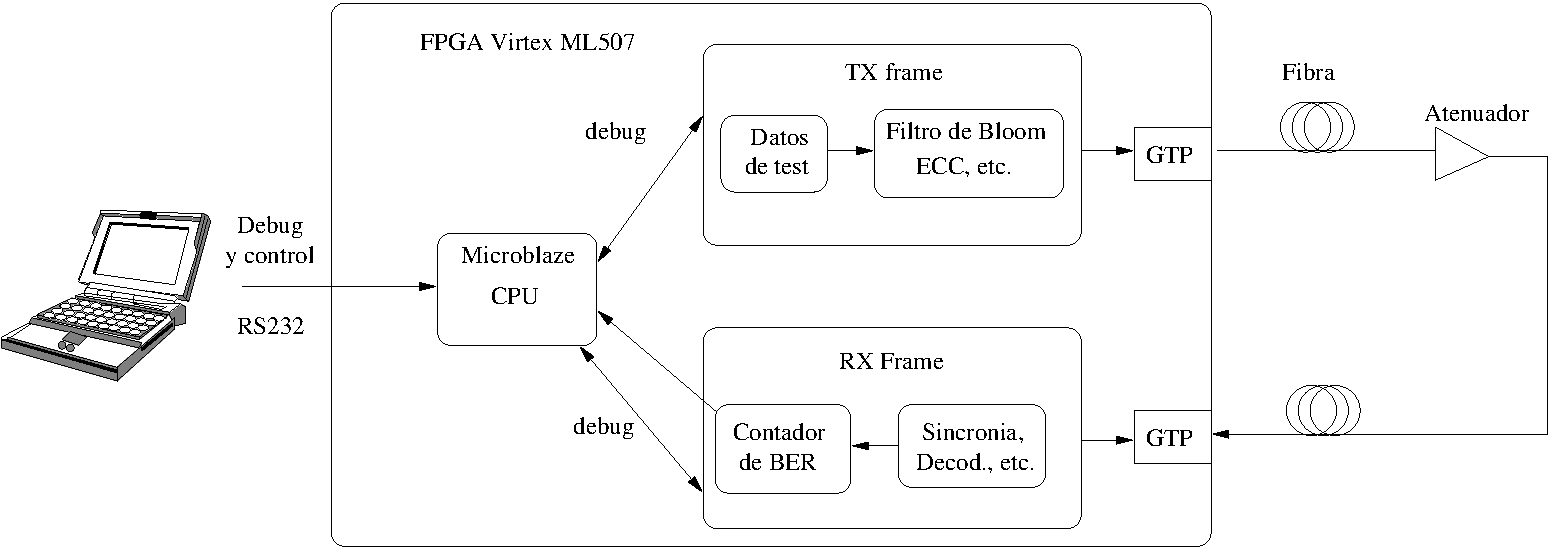
\includegraphics[width=6in]{graphs/fpgadesign.pdf}
\caption {Diseño de alto nivel sobre FPGA}
\label{fig:fpgadesign}
\end{figure}

% de confEUA.tex

\subsection{Transmisión a 9 Gbps con SFP+}
El montaje para la experiencia se realizó conectando el transceptor SFP+
al conector correspondiente en la placa de desarrollo ML-507 y un bucle de
fibra óptica ({\em loopback}), con el objetivo de realizar las
mediciones de BER. Luego, para realizar las mediciones con el
osciloscopio, se debe conectar el extremo de recepción de la fibra
óptica al osciloscopio. En este caso generamos el disparo del
osciloscopio mediante la señal de reloj del sistema (placa ML-507) que
se obtiene a través de los conectores SMA J12 y J13 (si bien es
diferencial sólo utilizamos uno de ellos).  Para la depuración y
configuración se utilizó la interfaz JTAG USB de Xilinx ``Platform Cable
USB II''.
\subsection{Configuración del reloj del transceptor}

La tasa de transmisión del transceptor GTX está dada por la
frecuencia de reloj de entrada $F_{PLL\_Clock}$, donde se transmite un
bit por cada semiciclo (la modulación es NRZ); entonces la tasa de
transmisión será
$R_{line}\mbox{[bps]}=F_{PLL\_Clock}\mbox{[1/s]} \times 2$.  La
frecuencia del reloj de entrada del PLL está gobernada por la ecuación
5-1 \cite[Pag. 88]{ug198}, que reproducimos a continuación:

\begin{equation}
F_{PLL\_Clock} = F_{CLKIN} \times \frac{PLL\_DIVSEL\_FB \times
DIV}{PLL\_DIVSEL\_REF}% \enspace
\end{equation}\\

donde las constantes $PLL\_DIVSEL\_REF = \{1;2\}$, $DIV = \{4;5\} $ y
$PLL\_DIVSEL\_FB = \{1;2;3;4;5\}$ son configurables por software;
mientras que la frecuencia base se configura con las llaves
SW6~\cite[Tabla 1-32]{ug347}: $
F_{CLKIN} (Mhz)= \{62.5;75;77.76;100;125;150;156.25;311.04;622.08\}$.


 Modificando los parámetros puede lograrse, en teoría, un amplio rango
de la frecuencias $F_{PLL\_Clock}$, pero de acuerdo a la documentación
del PLL \cite[Pág. 71]{ug366}~\footnote{La velocidad máxima no se
detalla en la documentación del GTX de Virtex5, pero si en la
documentación del Virtex-6, que excepto en el modelo HTX posee parámetros
similares.}, este tiene un rango de operación nominal desde $1.2$ a
$2.7$ Ghz en FPGAs de grado $-1$ tal como el que se encuentra en la
placa de desarrollo ML-507. Sin embargo en este artículo documentamos la
obtención y medición de velocidades de oscilación estables para el PLL
de hasta $4.5$ Ghz (lo que implica una tasa de transmisión de $9$ Gbps),
fuera del rango de operación especificado por el fabricante.

\begin{figure}[t]
  \centering
    %\includegraphics[scale=0.70]{plot.png}
    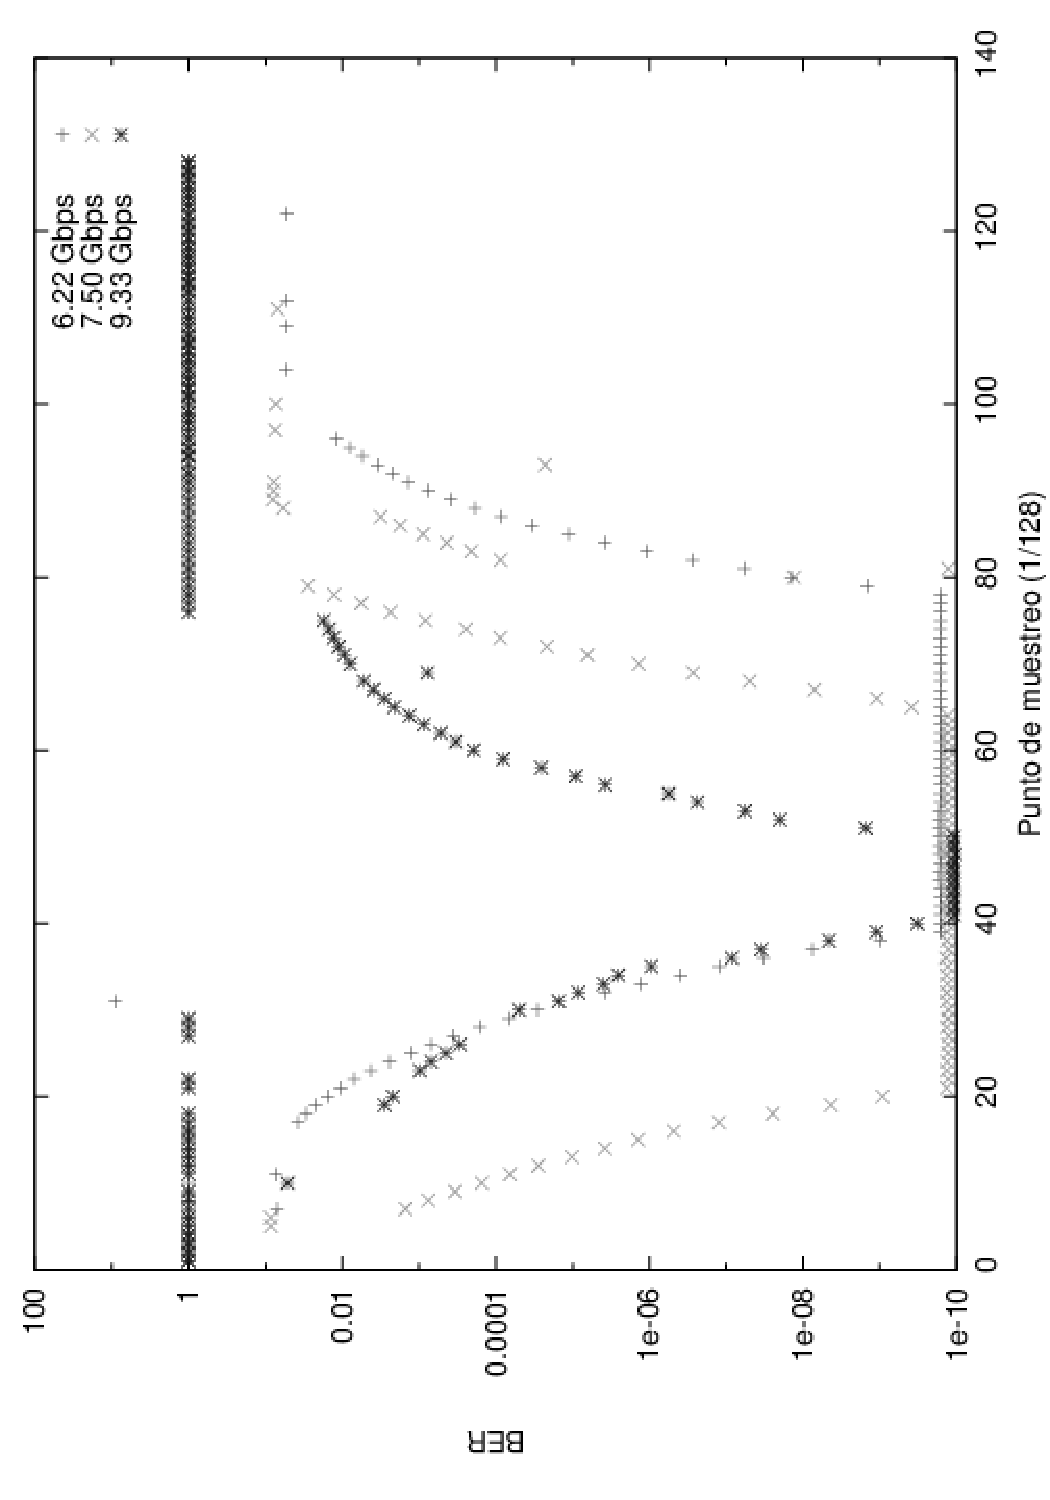
\includegraphics[width=3.5in,angle=270]{graphs/BER_sp_gray.pdf}
\caption {BER vs. punto de muestreo: como es esperable, el BER aumenta al samplear los extremos del bit, donde el diagrama de ojo es mas cerrado}
\label{fig:BERvsSamplingPoint}
\end{figure}

\subsection{características del transceptor de gigabit a altas velocidades}


\begin{figure}[!t]
   \centering
   \subfloat[Señal óptica a $4.5$ Gbps]{{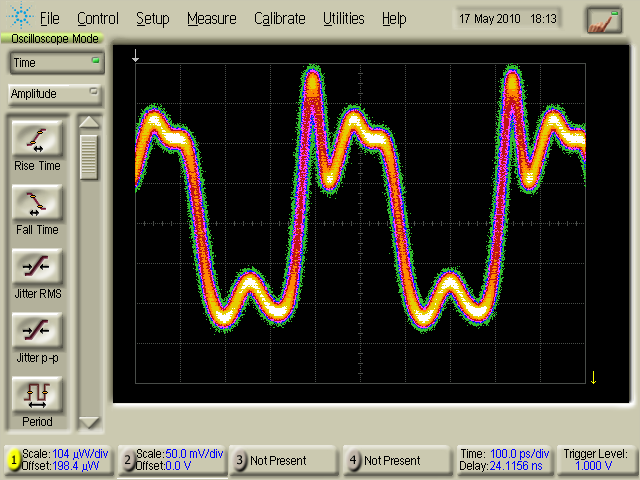
\includegraphics[width=0.45 \textwidth]{graphs/medicionesPaper/screen3.png} }}%
   \qquad
   \subfloat[Señal óptica a $6$ Gbps]{{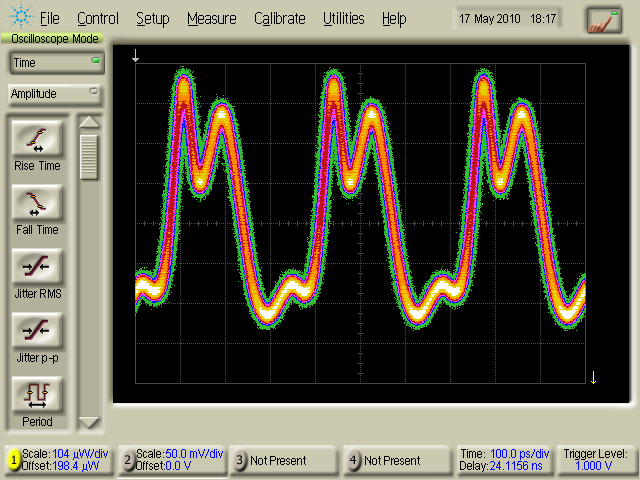
\includegraphics[width=0.45 \textwidth]{graphs/medicionesPaper/screen4.png} }}%
   \qquad
   \subfloat[Señal óptica a $7.5$ Gbps]{{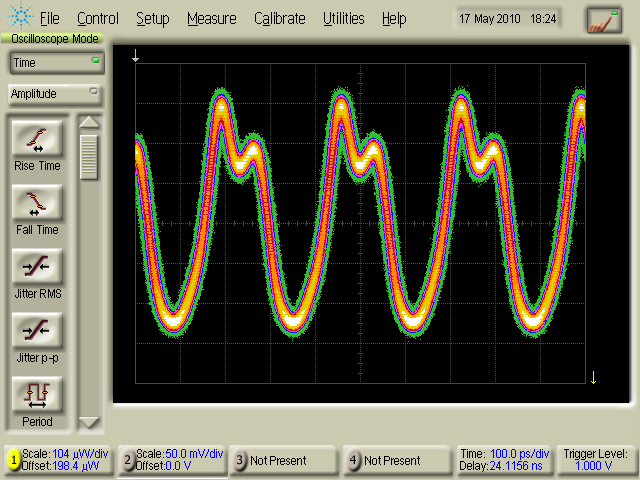
\includegraphics[width=0.45 \textwidth]{graphs/medicionesPaper/screen5.png} }}%
   \qquad
   \subfloat[Señal óptica a $9.33$ Gbps]{{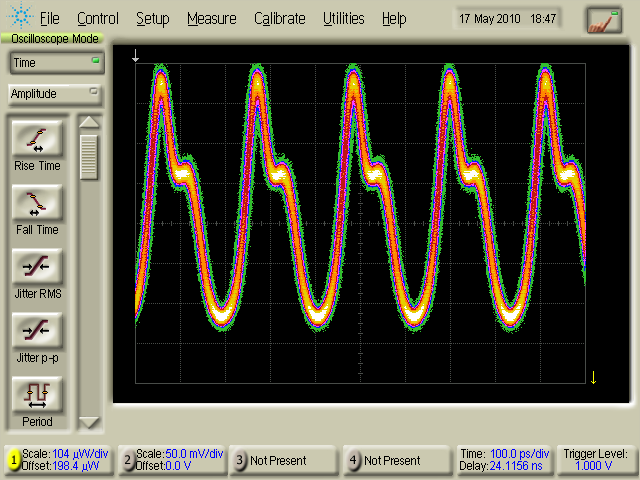
\includegraphics[width=0.45 \textwidth]{graphs/medicionesPaper/screen6.png} }}%
   \qquad
   \subfloat[Señal óptica a $12.44$ Gbps]{{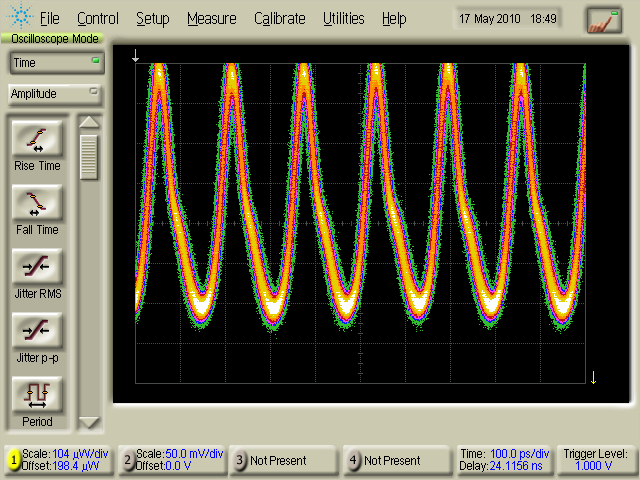
\includegraphics[width=0.45 \textwidth]{graphs/medicionesPaper/screen7.png} }}%
   \qquad
   \subfloat[Señal óptica a $12.44$ Gbps, transmisión 10110101010]{{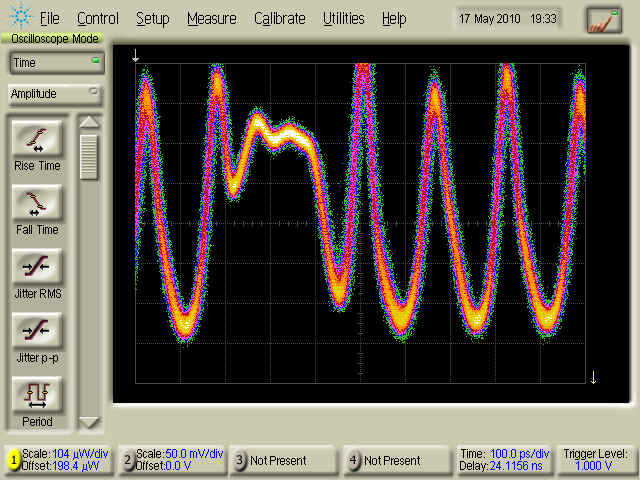
\includegraphics[width=0.45 \textwidth]{graphs/medicionesPaper/screen12.png} }}%
  \caption {Capturas de pantalla de la medición de la señal óptica a la salida del XFP variando la tasa de transmisión de $4.5$ a $12.44$ Gbps}
  \label{fig:ImgTasa}
\end{figure}





Las Fig.~\ref{fig:ImgTasa} muestran la evolución de la señal óptica producida a diferentes
tasas. Nótese que aunque el equipo puede generar señales estables de
hasta $12.44$ Gbps pero no puede recibirlas a esa frecuencia, por lo que las
mediciones de BER se realizaron solo hasta $9.33$ Gbps. Todas las señales
corresponden a la secuencia 10101010, excepto la última figura,
que fue generada con una secuencia distinta para demostrar el total
control sobre la señal generada. El transceptor posee la capacidad de
realizar una codificación 8B/10B adicional, pero para estas mediciones
ese módulo fue desactivado.
El punto de muestreo de la señal es importante, ya que si se elige correctamente se minimizará el BER, tal como lo muestra la Fig.~\ref{fig:BERvsSamplingPoint}, donde se aprecia como el BER es minimizado si el punto de muestreo cae exactamente en la mitad del bit. También en la misma figura puede compararse distintas tasas de transmisión y ver que las curvas de BER causadas por el punto de muestreo son diferentes para cada tasa. Esto es porque como puede verse en las Figs.~\ref{fig:ImgTasa}, a tasas elevadas el pulso del bit se deforma y el punto de muestreo óptimo se modifica, acompañando esta deformación del bit transmitido.


\subsection{Problema de linea desbalanceada y codificación 8B/10B}
La conexión eléctrica de la FPGA al Láser XFP debe soportar la transmisión de señales de 4 Gigahertz o mas, y puede verse como un canal con características de un filtro pasa-altas. Esto requiere que la señal este balanceada eléctricamente, por lo que deben codificaciones de balanceo para una correcta transmisión. Dichos algoritmos pueden ser el conocido 8B/10B u otras codificaciones, aunque 8B/10B tiene soporte de codificación/decodificación por hardware en el transceptor de gigabit de Xilinx.

El hardware de prototipado no permite implementar el algoritmo diseñado sin modificaciones. En la Fig.~\ref{fig:expansionbit} se aprecia una expansión progresiva a medida que el desbalanceo de la señal se hace mas pronunciado. Los efectos de la expansión del tamaño de bit son evidentes en la fig.~\ref{fig:ImgExpansion} donde las gráficas de potencia óptica ponen en evidencia la expansión e interferencia causada por una señal desbalanceada.
Efectivamente el receptor recibe hasta 3 ``unos'' por cada ``uno'' transmitido de manera desbalanceada, generando una interferencia que impide el funcionamiento del sistema.

\begin{figure}[t]
  \centering
    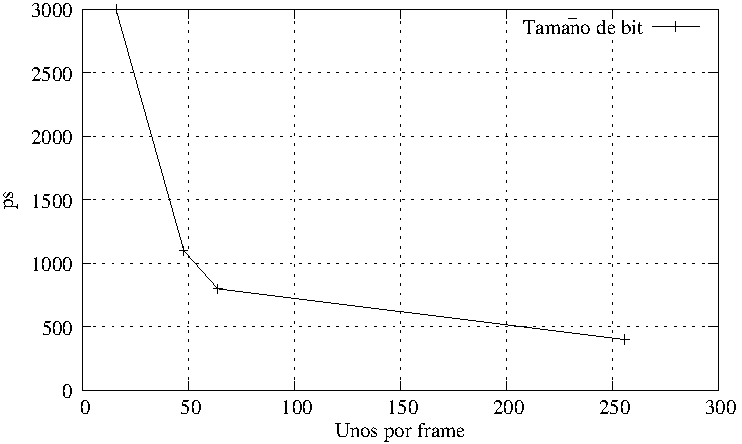
\includegraphics[width=4in]{graphs/expansionbit.pdf}
\caption {Se detalla la expansión del tiempo de bit en una señal desbalanceada a medida que la cantidad de unos por frame va disminuyendo. El tamaño de frame es de 512 bits, por lo que el mínimo de tamaño de bit esta con 256 unos por frame con una señal perfectamente balanceada. La tasa nominal es de 2.5Gbps}
\label{fig:expansionbit}
\end{figure}

\begin{figure}[!t]
   \centering
   \subfloat[Señal con 256 unos por frame (8B/10B), 400 ps por bit]{{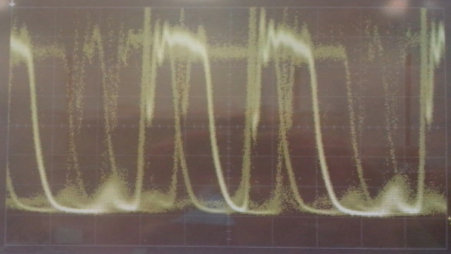
\includegraphics[width=0.45 \textwidth]{graphs/expansion1.jpg} }}%
   \qquad
   \subfloat[Señal con 48 unos por frame, 1100 ps por bit]{{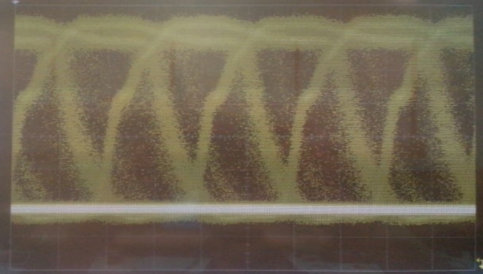
\includegraphics[width=0.45 \textwidth]{graphs/expansion2.jpg} }}%
   \qquad
  \caption {Señal de potencia óptica de un Láser XFP Sumitomo de 1330 nm. Se observa una expansión de bit cuando se reduce la cantidad de unos por frame, desbalanceando la señal. La tasa nominal utilizada es de 2.5 Gbps}
  \label{fig:ImgExpansion}
\end{figure}

Este desbalanceo se soluciona simplemente aplicando las codificaciones de balanceo a los datos antes de transmitirlos. Sin embargo, esta transformación es incompatible con el filtro de Bloom, ya que la interferencia de dos señales basta para eliminar la codificación y desbalancear nuevamente la señal. La solución definitiva es utilizar un hardware donde la señal no necesite balancearse, pero mientras tanto se opto por la siguiente solución para poder utilizar la placa ML507 y poder realizar mediciones sobre el protocolo: Al realizar las experiencias, uno de los clientes transmite su señal pseudoaleatoria superpuesta con una señal 8b/10b, por lo que la señal esta balanceada y es transmitida y recibida correctamente. Son los demás clientes los que transmiten una señal desbalanceada con muy pocos unos, causando solamente interferencias. La señal de estos clientes no puede recuperarse pero las mediciones son solamente realizadas sobre el cliente que esta balanceado, por lo que el sistema puede funcionar a la máxima tasa soportada por la FPGA (hasta 5Gbps) mientras que solo uno de los clientes pueda comunicarse y los demás actúen efectivamente solo como ruido.

\subsection{Sincronización a nivel de bit, word y frame}
\label{fpga:sync}
\begin{figure}[t]
  \centering
    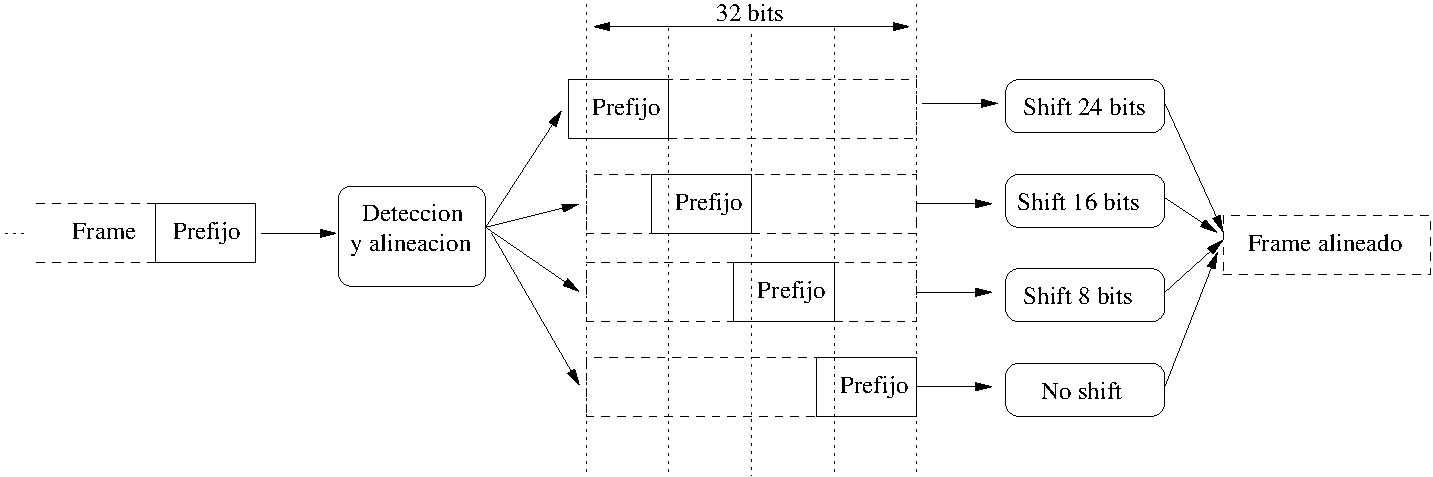
\includegraphics[width=6in]{graphs/optsync.pdf}
\caption {Flujo de datos en la sincronización óptica. El primer bloque, sincronización de bit alinea a un límite de byte, lo que resulta en cuatro posibles alineaciones distintas. El frame es luego es alineado a 32 bytes mediante desplazamientos o shifts.}
\label{fig:optsync}
\end{figure}


La sincronización no se trató detenidamente en la sección teórica de esta tesis ya que desde un principio se consideró como un tema ajeno a la misma. Sin embargo, para la implementación real es imprescindible obtener la sincronización entre los nodos que deseen utilizar un canal. Esto no es una tarea sencilla considerando que debe hacerse sobre un canal que contiene elevadas tasas de ruido.

La estrategia utilizada para la transmisión por medio óptico es utilizar el hardware de sincronización que posee el transceptor de multi-gigabit ya incluido en la FPGA. Este módulo \cite{ug198} denominado ``Comma Alignment and Detection'' se basa en la utilización de un prefijo o coma configurable que es una serie de bits (que puede ser de 10 o 20 bits de largo en el transceptor GTX) que se transmite cada vez que se desea sincronizar la estapa RX (receptor) con la TX (transmisor). Esta serie de bits es configurable pero es deseable que posea ciertas características como una alta auto-correlación, para optimizar su detección en el flujo de datos recibidos.
La sincronización se realiza en dos fases:
\begin{enumerate}
 \item El cliente que desea establecer un canal seguro envía el prefijo de sincronización (14 bits) y éste es detectado por el módulo de alineación del receptor. Este módulo alinea a nivel de bit y byte, o sea que garantiza que en el buffer de salida de 32 bits, el prefijo aparece en el bit 0, 8, 16 o 24 (Ver fig.\ref{fig:optsync}).
 \item Una vez alineado el prefijo en el buffer de salida, solo resta detectar en qué posición ha quedado y comenzar a leer el frame desde la posición siguiente. Esto se realiza en el código Verilog sintetizando cuatro detectores que simultáneamente testearan por cada posición y deciden en un solo reloj cual es la alineación correcta. Al ser solo 4 posiciones posibles, es una solución eficiente.
\end{enumerate}

En teoría, solo debería realizarse la sincronización al principio de las comunicaciones. En la práctica los relojes no son perfectos y es necesario sincronizar periódicamente. En la implementación óptica se envía el prefijo de sincronización al comienzo de cada frame.
Para evitar colisiones, el hardware de alineamiento se desactiva al detectarse una buena sincronización y se reactiva al finalizar la recepción del frame. Esta es una operación extremadamente rápida, recordemos que a una velocidad de 5Gbps, cada frame de 1024 bits tiene una duración temporal de 200 nanosegundos.

\section{Redes acústicas}
\label{redacus}
Debido en parte a la dificultad de implementación y depuración sobre la lógica de la FPGA, y la imposibilidad de realizar mediciones a muy altas velocidades, se propuso la implementación sobre un medio acústico como solución intermedia. Las señales acústicas se interfieren típicamente de manera aditiva y un modem acústico debe representarse como un canal binario simétrico en lugar de un canal-Z. Pero si utilizamos ciertas modulaciones, tales como OOK (on-off Keying) de manera que la frecuencia portadora sea varias veces mayor al ancho de bit, la interferencia entre bits tendrá siempre un efecto aditivo, mientras que los ceros no causan interferencia. Esto forma un canal-Z mediante el cual puede implementarse el sistema de comunicación segura descripto en esta tesis. Debido a las características de modulación necesarias, las velocidades de transmisión son muy bajas, ya que ancho de banda de un parlante o micrófono es relativamente reducido (de 2 a 15 khz) y la modulación OOK tiene una baja densidad espectral. 
No obstante es un excelente medio para realizar pruebas ya que pueden ser implementadas totalmente via software, y puede ser utilizado en todas las aplicaciones que no requieren elevadas tasas de transmisión.

\subsection{Modulación}
% de newJIS_140512
El medio de transmisión acústico utiliza ondas de presión en lugar de electromagnéticas pero las técnicas de modulación que pueden utilizarse son las mismas.
Sin embargo, no todas las modulaciones siguen el comportamiento de canal Z descrito en la Sección \ref{canalZ}.
La modulación On-Off Keying (Un caso especial de modulación ASK, Amplitude Shift Keying), es uno de los tipos de modulación que permite implementar un canal Z sobre un medio acústico si se utiliza sobre cierto rango de parámetros. Utilizando transductores (micrófonos y parlantes) comerciales del tipo presentes en la mayoría de los dispositivos móviles probados, la frecuencia de portadora puede variar de 10 Khz a 16 Khz. Se obtienen resultados buenos con una tasa de transmisión de 1000 bps al nivel de frame. En los experimentos que se detallaran en las secciones siguientes, el retraso (delay) o tiempo que le lleva a un bit atravesar la red, fue extremadamente alto debido a una combinación de baja velocidad de transmisión y la necesidad de un buffer muy grande (1024 bits) necesario para la utilización del esquema de corrección de errores seleccionado (Reed-Solomon 223/255). Si bien aumentar la velocidad de transmisión no es sencillo, modificar el algoritmo de corrección de errores o sus parámetros (Por ejemplo, utilizar algún esquema tipo BCH [12]) podría reducir el retraso de datos drásticamente.

Como técnica de ``pulse-shaping'' se utiliza un simple filtro FIR pasa-banda a la salida de la etapa de modulación, así como también en la entrada de la etapa de demodulación. Este filtro además de reducir el ancho de banda utilizado, ayuda a rechazar interferencias.
Adicionalmente un duty-cycle de 50\% demostró ser el óptimo para la modulación.
%On-Off Keying modulation of sound waves, following the Z-channel interface model described in Section 2.2., encode the transmitted bits as pulses. Carrier frequency can vary from 10 kHz to 16 kHz. Good results can be obtained with a rate of 1000 bps at frame level. In experiments, delay (the time for a bit to traverse the network) was very high, due to Reed-Solomon 223/255 coding, a frame to support up to 16 users and the low capacity of the physical media. A more sensible choice of FEC algorithm (like BCH [12]) could drastically reduce data delay. 

%Simple pulse shaping is realized using a pass-band filter at the output of the modulation and also at the input of the demodulator. This filter also helps reject unwanted interference.
\subsection{Sincronización}
% de newJIS_140512

\begin{figure}[t]
  \centering
    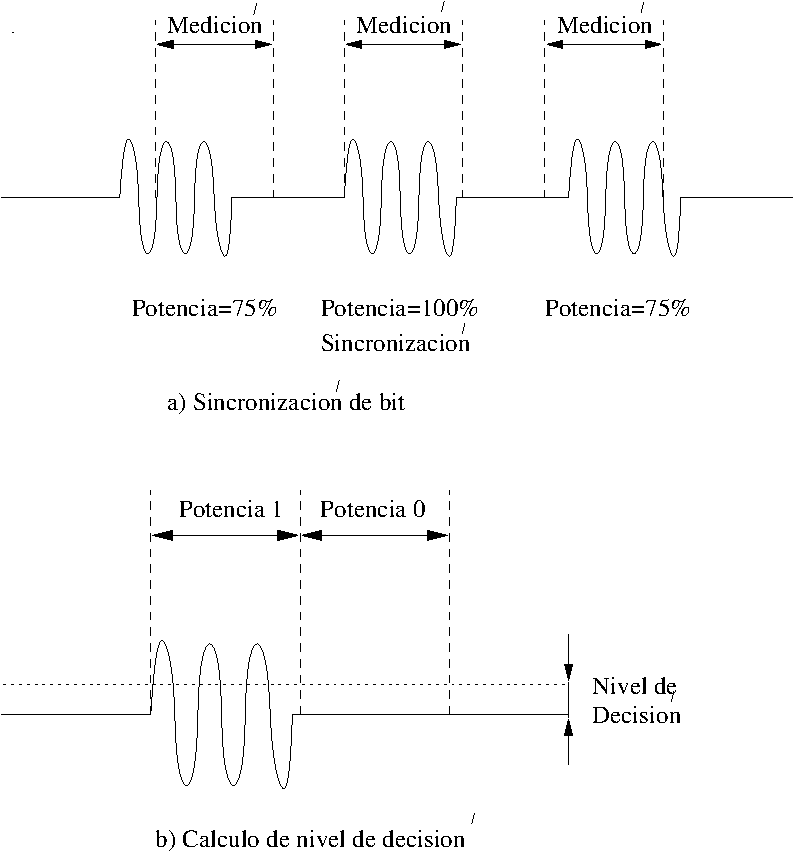
\includegraphics[width=4in]{graphs/acusync.pdf}
\caption {Sincronización acústica. En la figura a) se recorren consecutivamente todas las posibilidades hasta encontrar la mayor potencia de bit, que corresponde a la mejor sincronización. Luego, en la figura b) se calcula el umbral de decisión.}
\label{fig:acusync}
\end{figure}

Como se desprende de la descripción del canal de comunicaciones, la sincronización entre el transmisor y el receptor es esencial para la correcta decodificación de la información. 
En el caso del medio óptico la sincronización de bit y word (16 bits) debe realizarse a tasas tan elevadas que requiere necesariamente soporte de hardware por parte del transceptor.
Sin embargo a las reducidas tasas (1000 bps) utilizadas en el canal acústico permiten realizar una sincronización por software sin ningún soporte de hardware adicional. 
El método es muy similar al utilizado en el canal óptico: Un patrón inicial de sincronización es enviado, para que el receptor pueda realizar un ajuste de parámetros tales como fase y umbral de decisión (Ver Fig.~\ref{fig:acusync}). La deriva y fluctuación del reloj del sistema (drift y jitter) no son significantes a esta baja velocidad de transmisión por lo que no se requiere corrección de ningún tipo, haciendo que la Implementación del modem por software sea muy sencilla.
Ciertos parámetros si bien son inicializados en la etapa de sincronización, son por naturaleza dinámicos y se ajustan periódicamente, como por ejemplo el umbral de decisión, que es recalculado a partir de un promedio de los datos de entrada. La fase es también corregida utilizando los datos de entrada como referencia. Notar que este método de sincronización simple permite detectar el comienzo de frame a su vez que se alinea a nivel de bit; ambas alineaciones son necesarias en cada comunicación (pero la alineación de frame solamente entre los ONUs comunicantes). Adicionalmente, una vez comenzada la transmisión, los datos serán indescifrables gracias al algoritmo CDMA de time-hopping guiado por un CS-PRNG.

%As it follows from the description of the communication channel, synchronization between the transmitter and receiver is essential for the correct decoding of information. For this purpose, an initial synchronization pattern is sent, so the receiver can adjust parameters like phase and decision level (see Figure 3). For the data bits transmission a duty cycle of 50\% showed in our experiments an enhanced detection. Clock drift and jitter are not significant at this low transmission speed and so no correction is required, making the software modem implementation very simple. Decision level is dynamic, meaning it is constantly re-calculated from averaged input data. The receiver symbol phase is also corrected using the input data as reference. Notice that this simple synchronization method allows detecting the frame start as well as the bit slot; both are needed at every communication. Moreover, once the data began to be transmitted, the communication becomes indecipherable thanks to the CS-PRNG.


\subsection{Medición multi-usuario}

Todas las mediciones fueron realizadas a una tasa de 1000 bps, utilizando una señal portadora acústica de 16 kHz, que se encuentra en el límite auditivo de la mayoría de los adultos de más de 40 años \cite{gordon2005hearing} aunque también es posible que ciertos parlantes tengan problemas a esta frecuencia, en cuyo caso puede reducirse y utilizar una portadora de 12 kHz.
La cantidad total de datos transmitidos por canal fue de 4096 bits en cada medición. El volumen de la señal fue configurado al máximo para cada dispositivo, mientras que la amplificación de entrada de la señal obtenida por el micrófono fue optimizada en cada caso para obtener el menor BER.
Con el modulador y circuito de sincronización implementados, el sistema opera con tasas de error aceptables con una separación máxima entre nodos de 1 metro, una distancia que normalmente excede la existente entre un terminal móvil (Celular, etc.) y una computadora fija en el mismo escritorio (Ver Fig.~\ref{fig:acudist}). Aún para un alto número de clientes simultáneos (>10) el sistema no presenta altas tasas de error o ancho de banda reducido, como puede verse en la Fig.~\ref{fig:acumult}.
En las pruebas con el software actual, el retraso del canal es de mas de 60 segundos, excesivo para muchas aplicaciones que no necesitan alto ancho de banda pero requieren un corto tiempo de respuesta (por ejemplo, aplicaciones bancarias). El retraso puede ser disminuido de dos maneras: 
\begin{enumerate}
 \item Decrementando la cantidad máxima de clientes simultáneos soportados por el sistema.
 \item Utilizando algoritmos de ECC de bajo retraso, tales como BCH, ya que actualmente el retraso esta causado por el algoritmo de Reed-Solomon que requiere llenar un buffer de 256 bytes (2048 bits) antes de poder comenzar la decodificación.
\end{enumerate}

\begin{figure}[t]
  \centering
    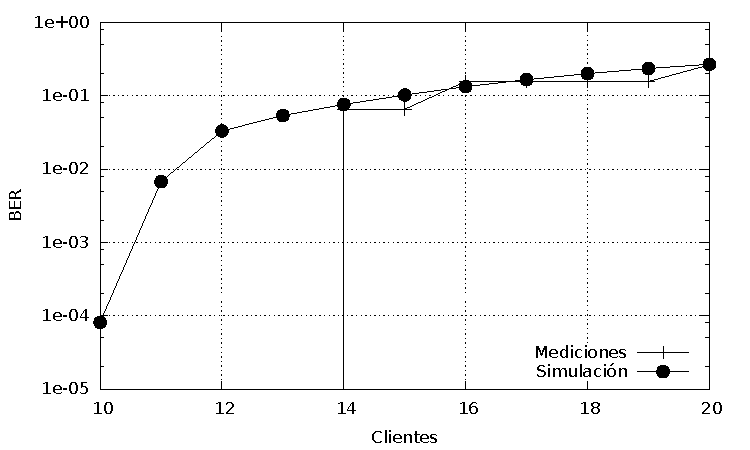
\includegraphics[width=4in]{graphs/medidas_clientes_JIS-fig6.pdf}
\caption {Multi-usuario: BER del enlace entre dos laptops (Lenovo T420 y Lenovo X60), una de ellas simulando varios nodos}
\label{fig:acumult}
\end{figure}


% De JIS2014MathType.pdf
%All measurements were conducted at a rate of 1000 bps, with the carrier signal at 16 kHz. The total data trans-
%mitted was 4096 bits. Output volume was set at the maximum possible for each device, while the input amplifi-
%cation was optimized for each measurement.
%We measured that the system operates with acceptable error rates for links of up to 1 meter, a distance usually
%exceeding that between a mobile terminal (phone, etc.) and a fixed computer placed in the same desk (see Fig-
%ure 7). Even for a high number of concurrent clients (>10) the system does not present high error rates or re-
%duced bandwidth, as can be seen in Figure 6.
%Although in the present test channel delay was longer than 60 seconds, excessive for some applications re-
%quiring short response time (e.g. banking transactions), this parameter can be reduced by decreasing the maxi-
%mum number of simultaneous users supported by the system and using a lower-delay interleaver and an outer
%error correction algorithm like BCH
%

\subsection{Medición a distinta separación}

\begin{figure}[t]
  \centering
    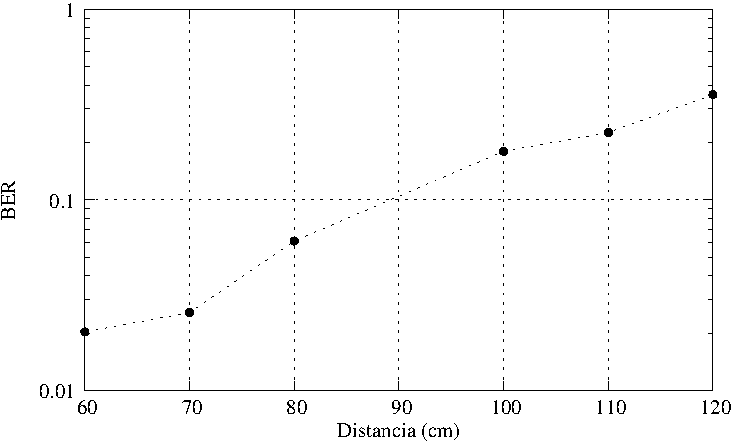
\includegraphics[width=4in]{graphs/mediciones-distancia-fig7.pdf}
\caption {Distancia: Enlace entre una Laptop (Lenovo T420) y un celular (HTC Status) presenta errores detectables solo cuando se supera 60 cm de separación.}
\label{fig:acudist}
\end{figure}

Las comunicaciones acústicas utilizando como portadora un tono de 12 kHz son muy susceptibles al ruido ambiente. Un enlace acústico con 50 cm de separación entre un Laptop Lenovo T420 y un celular HTC Status sufrió mas de un $15\%$ de BER con solo una ligera interferencia (como por ejemplo golpear una mesa cercana). Esta observación motivo el uso de la frecuencia mas alto posible. Una portadora de 16 kHz presentó el mayor rango de compatibilidad entre los dispositivos testeados, algunos de ellos demostraron no poder emitir audio a frecuencias mayores.
Independientemente, algunas mediciones fueron realizadas a mayor frecuencia en dispositivos que lo soportaron. Por ejemplo, los parlantes de una Laptop T420 y otra Laptop Lenovo X60 fueron capaces de establecer un enlace utilizando como portadora un tono a 19.2 kHz, aunque solo en cortas distancias (20 cm). De todas formas, esta frecuencia de portadora permitió mayor ancho de banda en el enlace (2000 bps en lugar de 1000 bps) con la misma tasa de error.
La señal acústica modulada puede causar molestias a personas o animales cercanos. Distintos tonos de portadora causan distintos efectos y niveles de molestia, aunque este último parámetro es subjetivo. La portadora de 19.2 kHz fue descrita como no audible, mientras que la portadora a 16 kHz y 12 kHz son claramente audibles. Se notó que el volumen del sonido modulado y las molestias asociadas al mismo aumentan con el numero de clientes simultáneos transmitiendo en el medio.

% De JIS2014MathType.pdf
%Communications using a 12 kHz tone carrier were extremely susceptible to ambient noise. Indeed, a 50 cm
%link between a laptop Lenovo T420 and a HTC Status phone suffered an excess of 15% BER with slight noise
%%interference (like bumping on a nearby table). This observation motivated the use of the highest attainable fre-
%quency. A 16 kHz carrier provided the widest range of compatibility among tested devices, because some of
%them could not emit at higher frequencies.
%Tests were also done at higher frequencies for capable devices. For instance, laptop speakers in Lenovo T420
%and Lenovo X60 laptops proved capable of establishing a link at 19.2 kHz, but only for very short distances
%(20cm). Nevertheless, this carrier frequency allowed a faster link (2000 bps) with the same BER.
%The modulated sound signal can represent a nuisance to nearby persons and animals. Several different carrier
%frequencies were tested as a way to evaluate the level of discomfort. The 19.2 kHz carrier signal was perceived
%as almost non-audible, with 16 kHz being clearly audible for most people and the link at 12 kHz being the most
%uncomfortable. It should be noticed that loudness and hence discomfort increase with the number of simultane-
%hous users.
%
